\chapter{Methodology}
\label{chap:methodology}

\todo{write a short recap of the methodology as introduction}
This project followed a user-centred design methodology to structure the design process to build the chatbot prototypes. The process towards building the prototypes and the evaluation will be used to answer the research questions:

\begin{enumerate}
    \item How can we design chatbot personalities to guide the design process of a chatbot interface? 
        \subitem a) Can personality be used as a stable pattern to guide the design \subitem    process of chatbot interfaces?
        \subitem b) Which elements must be considered to inform a chatbot personality?
        \subitem c) What components needs to be in place for a chatbot personality to \subitem  meet user needs and expectations?
    \item Will chatbots with a defined personality improve the user experience of chatbot interfaces?
\end{enumerate}

The design process will help answer the first research question and sub-questions. As there are no precise design methodology to build user-centred chatbots, with a basis in personality, the researcher has combined techniques from user-centred design, branding, and personality theory in order to form a personality framework for chatbot interfaces. This second research questions will be answered through the experiment laid out in this chapter. First, the personality framework and design process will be explained, second the experiment setup and data collection forms will be laid out in depth.

\vspace{5mm} %5mm vertical space

\subsection{Brand, Domain, and Usage}

To build the chatbot prototype, test the personality framework, and follow a user-centred design approach, the chatbot domain will be based on a real brand. There are no formal collaboration with this brand, therefore it will be anonymised in this thesis. It was necessary to use a real life example to base the prototype on in order to show how the chatbot personality represents the brand's tone of voice, mission and values. This also informed user personas, and suitable users for the chatbot prototype to model the personality on. In addition to this it also informed the role and job the chatbot should have to add value to users and support the mission of the brand.

The chatbot prototype will be used to further the mission of the brand which is to increase the consumption of fruits and vegetables and reduce food waste. 

\subsection{User group}

The intended user group for the chatbot prototype are between the ages of 25 to 40, aiming at young parents with young children. Research have found that this age group eats less fruits and vegetables and waste the most food 
\todo {add citation}. Therefore, to support the brand's mission of increased consumption of fruit and vegetables, the chatbot will focus on this target audience. This group usually have hectic days where healthy eating and activity can be difficult to maintain, and they are also in charge of their children’s diet and activity levels as well. As learning good habits starts when we are children, parents have a major impact in regards to teaching children the right habits. This shows that this group in particular are in need of a service which can help them cook healthy meals for themselves and their families, receive assistance to find easy and economical ways to add more nutritious produce to their meals, which will contribute to less food wasted.

\section{Personality Framework}

The design process, UCD approach, helped form the requirements for the system, define system goals, and use cases. In addition it allowed for valuable insights regarding the users, their needs and frustrations with current solutions. This was necessary to understand the role of the chatbot, and which tasks were necessary for it to do. However, while we know what it needs to do, how can we script the conversation, the different intents, in which the users will have when addressing the chatbot? 

In order to write the chatbot conversation flow, one must be able to understand how the chatbot should behave, and how this behaviour, or personality, best suits the users. To build the personality framework the researcher identified four components that the chatbot personality must be based on:

\begin{enumerate}
    \item A deep understanding of the users and their needs %see whether the inspiration phase should be located here
    \item The brand mission, goals and values
    \item The role/job of the chatbot
    \item An appropriate personality model
\end{enumerate}

These four conditions describes four questions that designers must have the answer to in order to have the necessary components to build the chatbot personality.

\vspace{5mm} %5mm vertical space

\subsection{Design process to determine user needs}

To meet the first component; to build a deep understanding of the users and their needs, a user-centred design approach was followed to gain insights into the needs and inform the requirements of the chatbot prototypes. The UCD process was divided into the stages of:  1) inspiration 2) ideation 3) implementation (See Figure 3.0, IDEO.org, 2015). According to \cite{Gould1985} there are three key principles of UCD: an early focus on users and tasks, empirical measurement of product usage, and iterative design. The three stages will therefore all follow the key principles of UCD, where the first stage (inspiration) will focus on user and domain research, ideation will focus on designing the elements of the chatbot prototype, and implementation will focus on the final prototype which will be used to evaluate the design process, the personality framework, and whether personality design benefits the user experience. As a UCD approach is characterised by empirical measurement, iterative design, and focus on users, each deliverable will be empirically tested through user testing techniques in iterations to inform the final prototype.

\vspace{2,5mm} %2,5mm vertical space

    \subsubsection{User interviews}
    
   All the stages of the design process followed a strict user-centred design methodology. The inspiration phase focused on gathering insights into the domain at hand. This included conducting a brand analysis of the available content in order to inform the mission statement, values, goals and target audiences. In addition, secondary research was gathered in order to understand trends, causes and action-plans regarding increasing healthier lifestyles and waste less food.
   
   Once secondary knowledge had been collected, a series of interviews was conducted in order to understand the experiences of the users, how do they view their intake of fruit and vegetables, what obstacles do they face, and why they think they are not eating healthy enough. Eight users were recruited, or four couples, in the ages of 29 to 36, four mothers and four fathers. All four couples had two children in kindergarten and/or early elementary school age. Six of the participants works full time, while one mother was on maternal leave as the interviews were conducted. Two participants, one male and one female, were part-time workers and/or students at the time of the interviews.
   
   The interview guides prepared were semi-structured and aimed at mapping the daily routines, views, habits, pains and frustrations of the users during an average week. In particular the interviews aimed to see how parents assess their own eating and activity habits, and whether they are aware of food waste occurring and if so why. The interview guide can be found in Appendix XX. 
   
   The findings from the interviews were summarised to inform a PACT analysis (appendix XX), to give an understanding of the current state of the services and digital channels of the brand in question and the user group.

\vspace{2,5mm} %2,5mm vertical space

    \subsubsection{User Personas and User Scenarios}
    
    In the ideation phase the researcher created user personas, based on findings from the interview and the PACT analysis. To understand the requirements of the system, the user personas describes which goals the users wish to meet using the chatbot, their frustrations and pains and motivations for using the chatbot. Once the personas had been formed, findings from the inspirations phase were used to develop user scenarios --> conceptual scenarios --> concrete scenarios --> use cases. These can be found in Appendix XX.
    
    %show flowchart of how to use scenarios
    
\vspace{2,5mm} %2,5mm vertical space

    \subsection{The Brand Mission, Goals, and Values}
    To design a chatbot that conforms to the brand it represents, the brand image was analysed and defined. The mission statement was identified, the company and core values was defined, and a tone-of-voice analysis was conducted.
    
\vspace{2,5mm}
    
        \subsubsection{Mission statement and core values}
 
        The brand describes itself as having a broad social responsibility. They supply fruits and vegetables, with suppliers on all continents providing products from all over the world. Freshness is the top priority and high quality. In addition to providing fresh produce, the brand recognises having a fair and sustainable business model, which extends to proper nutrition, increased activity, and societal and environmental responsibilities. Their goal is to increase the consumption of fruit and vegetables, therefore in addition to supplying fresh produce, they take an active role in increasing knowledge and engagement regarding healthy lifestyles and positive societal development.
 
\vspace{2,5mm}
  
        \subsubsection{Mission: Fresher and healthier}
        Taken a society position in the  market that contributes to increased focus on healthy diets and physical activity
        A driver and pioneer for sustainable development regarding the environment and societal responsibility within the company’s product area
        
\vspace{2,5mm}

        \subsubsection{Brand Values}
        
        To create value for our consumers/customers is our driving force throughout the business. The conduct of employees are characterised by the values stated in Table \ref{table:1}:
        
    \begin{table}[h]
    \begin{tabular}{ |p{9cm}||p{5,4cm}|  }
     \hline
     Internal Values & Core Values \\
     \hline
        Team spirit & Vital \\
        Courage to do the right thing: Openness, honesty, probity & Current\\
        Compassion: mutual respect, care, and tolerance & Fresh \\
        & Daring    \\
     \hline
    \end{tabular}
    \caption{Internal values and core values}
    \label{table:1}
    \end{table}

        \subsubsection{Tone of Voice analysis}
    
        If the chatbot are to be perceived as an extension or continuation of the brand, it must adhere to the brands tone-of-voice. Tone-of-voice is defined as a brands personality, communicated through its written communication as well as the visual communication. Norman \& Nielsen defined a framework to determine tone-of-voice based on 4 dimension: funny vs. serious, formal vs. causal, respectful vs. irreverent, enthusiastic vs. matter-of-fact.
    
        \begin{figure}
            \centering
            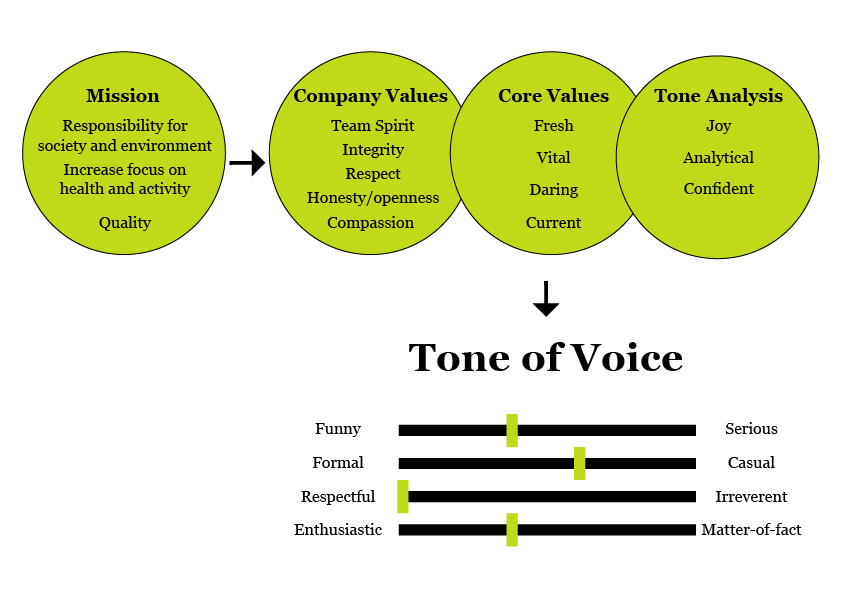
\includegraphics[width=\textwidth]{figures/Tone-of-voice.png}
            \caption{This figure shows how the tone-of-voice was defined by understanding the mission, the values and conducting a tone analysis of the written copy}
            \label{fig:tov}
        \end{figure}
    
        Figure \ref{fig:tov} shows how the tone-of-voice was determined by assessing the mission statement, the company's values inwards and outwards, and through a tone analysis. The tone analysis was conducted using the IBM tone analyser tool, the analyser assessed the written copy found on the brands website. Their tone-of-voice as reflected in their copy is more serious than funny, but not too serious as the tone is also a nice in-between of formal and casual. Their tone is very respectful, which follows their core values of tolerance and respectfulness. Lastly they are leaning towards more enthusiastic than matter-of-fact as they carry a very positive and joyful view of the future and their path to fullfil their goals.

\vspace{5mm}

    \subsection{The Chatbot Role}
    
    The user-centred approach identified the two most important jobs the chatbot could do that both furthers the goals of the brand and add value to the users: increase the consumption of fruits and vegetables, and reduce food waste. Therefore, the job of the chatbot agent is to \textit{assist} users to help them take healthier choices for their family and \textit{motivate} them to successfully implement these changes. The chatbot is there to assist and guide the users, with the long term goal of successfully implementing a fresher and healthier lifestyle and reduce food waste. 
    
    To achieve this the chatbot will help parents plan their dinners for the whole week, assist with the shopping and make recommendations based on ingredients they have in house and leftovers. In addition to this the chatbot encourages parents to inform the chatbot about what they have eaten so far, what was a success and what wasn’t so that the chatbot can learn which items are not eaten, are wasted and instead offer healthy alternatives that will be eaten rather than wasted. 
    
    Assistants and motivators have specific traits in which they need to have in order to be successful in their role (see table \ref{table:2}).
    
\vspace{2,5mm}

    \begin{table}[h]
    \begin{tabular}{ |p{7,2cm}||p{7,2cm}|  }
    \hline
    Assistant & Motivator \\
    \hline
        Professionalism & Give praise and encouragement \\
        Collaborators & Treat clients as equals \\
        Outstanding organisational skills & Show trust \\
        Excellent communication skills & Communicate and set goals \\
        Willingness to go the extra miles & Be attentive \\
        Problem-solver & Allow mistakes \\
        Proactive & Be pleasant \\
        Respectful & Ask for feedback \\
        & Keep others informed \\
        & Don’t micromanage \\
    \hline
    \end{tabular}
    \caption{Desirable traits for Assistants and Motivators}
    \label{table:2}
    \end{table}
 
    The traits of the assistant will be reflected in the way the chatbot handles its job. Through AI and NLP capabilities, as well as connection to necessary APIs, will the chatbot be able to complete necessary tasks and incorporate “hidden/invisible” features that will help users achieve their goals. As for the motivator traits, this will be reflected in how it encourages/motivates users, the language its using, and its behaviour (prompts, affirmations, tips). Therefore the chatbot role will be reflected by its external traits (motivator) and its internal traits (assistant).
    
\vspace{5mm}

    \subsection{Personality Trait Model}
    Once the brand mission, core values, understanding of user needs, and the chatbot role have been identified, designers should find an appropriate personality trait model to help put together a dynamic personality for the chatbot. It is important that this model will be used to place the desired personality within a framework, this is to benefit the designer when designing a consistent personality. 
    
    It is not the goal of this thesis to assess whether the designed personality is consistent with the chosen trait model, or to assess the personality of participants. The trait model is only used to guide the design of the chatbot personality, and to help in evaluating desirable traits for the specific chatbot agent. 
    
    The chosen personality model to model this chatbot's personality was the five factor model. As explained in section 2.3.2, this personality trait model is widely know, and based on lexical data used by humans to describe personalities. These traits have been mapped out and organised into the five factors, and as the traits are identified by the words we use to describe them, it will be an appropriate model for a linguistic interface such as a chatbot.
    
\vspace{5mm}

    \subsection{The Chatbot Personality Description}
    The final chatbot personality therefore were based on identified user needs and user personas, the brand image and tone of voice, and the identified role of the chatbot. This information was used to model the desirable traits and quirks of the chatbot personality, and the five factor model was used as reference to model the personality. The personality includes the traits shown in Figure \ref{fig:characteristics}. The role and character description is laid out in next two sections; both descriptions are based on the user research in regards to how the chatbot's tone and tasks are handled to support the needs and goals of both mothers and fathers.
    
    \begin{figure}[h]
            \centering
            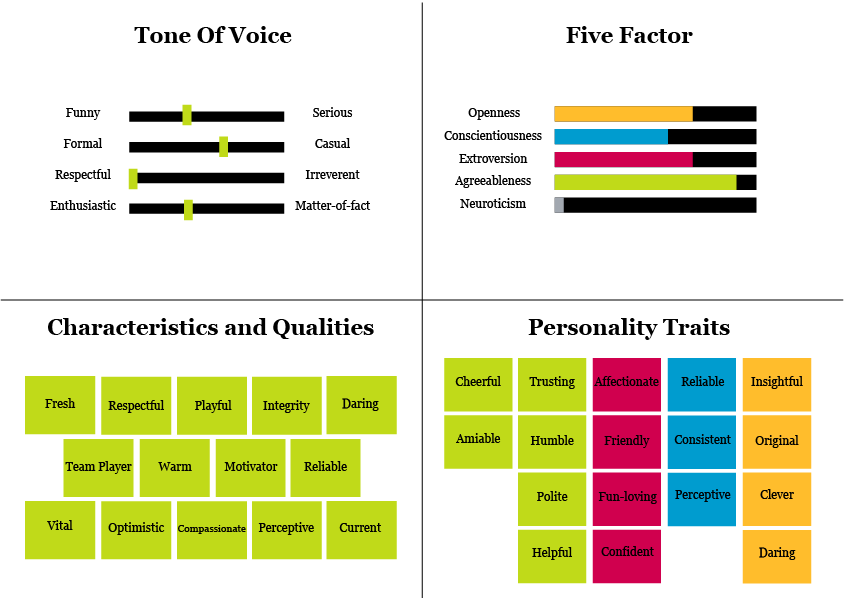
\includegraphics[scale=0.5]{figures/Defined_characteristics_and_traits.png}
            \caption{The defined tone-of-voice, five factor personality traits, characteristics and qualities}
            \label{fig:characteristics}
        \end{figure}
    
    \subsubsection{Role description}
    The chatbot has been given the name Bella. She works as a dinner planner, helping parents plan meals for the whole week. Her recipes helps parents eat a healthy and balanced diet focusing on increasing the consumption of fruits and vegetables. Bella is personalised to each specific family as she knows and learns over time what they prefer to eat, what they dislike, any known allergies they might have, and who makes up the whole family. Her mission is to increase their health, while also taking an environmental and economical approach to dinner planning; keeping track of what food they have at home, base recipes on ingredients that needs to be used up and providing parents with shopping lists. It is important that Bella works to motivate mothers and fathers towards their goals, and does so in a supportive fashion. Her role as assistant makes sure that she is trustworthy, reliable and efficient.
    
    \subsubsection{Character description}
    Bella is designed to act and look about the same age as her target audience, she is an assistant and motivator for both mothers and fathers. However, her personality is modelled to be that of a supportive friend for mothers, helping her with cool new tricks and emotional support, by using a cheerful and playful tone. This is because mothers are more likely to use Bella often throughout the day, to log meals, ask for help and tricks. Fathers on the other hand will most likely use Bella mainly when they are in need of reminders, accessing shopping lists and recipes. Therefore Bella acts efficiently and to the point, while also providing a helpful and supportive tone. She is cheerful, youthful, and fun-loving, while also being reliant, consistent, efficient and trusting. Bella is a team player, and works to support great collaboration between the mother and father. 

\vspace{5mm}

    \subsection{Prototype \& Conversational Design}
    The chatbot prototype was built using the Chatfuel bot builder platform. The conversation design was written by mixing a user scenario technique with mind-mapping tools, such as Xmind, to map out the different chatbot skills, user intentions, and conversation flows. To improve the AI of the chatbot, the researcher wrote more than 300 unique training data per chatbot skill.
        
\vspace{5mm}

    \subsection{Avatars}
    The literature review investigated how humans perceive the various types of conversational agents, and found that anthropomorphism can benefit how a personality is perceived, and that a consistent personality dictates which characteristics humans assign to a chatbot in which they anthropomorphise. The literature review also discussed humanness as it related to human capabilities and physical characteristics. The review found that chatbots with a high levels of humanness increases trust and familiarity, while also providing a more natural interaction with humans. The latter is explained by that humans know how to interact with other humans, therefore will assume that a chatbot will interact like a human if looking human. 
        
    Because of this, the chatbot avatar will have a human appearance. This chatbot is taking on human tasks and is to be perceived as a human. However, research have found that too human might have a negative effect on human perception which is why the chatbot will be portrayed as an illustrated character rather than a realistic human. This will make clear the distinction that the chatbot is not a human, while incorporating high levels of humanness simultaneously.
    
\vspace{5mm}

    \subsection{Chatbot B - the other chatbot}
    As there is no baseline data available to compare the personality effect against, another chatbot version was also created in order to assess and compare the user experience of each chatbot version. While the chatbot described above (Chatbot A) has been given a human personality based on the brand and users, Chatbot B has been designed to appear less human. Chatbot B cannot be defined as having "no personality", as even a "machine-like" behaviour can be defined as a personality type. Instead Chatbot B has been designed to be mainly task-oriented, providing the same service and completing the same task as Chatbot A, but in a machine-like way as shown in table \ref{table:3}.
    
    \begin{table}[h]
    \begin{tabular}{ |p{3cm}||p{5cm}||p{5cm}| }
     \hline
        User Expressions & Chatbot A & Chatbot B \\
     \hline
        What should I cook for dinner tonight? &    Cool cool;) What are you in the mood for?   & Do you have a preference? \\
     \hline   
        Something that's quick to make &   In a hurry today huh? Here is a selection of 3 meals that takes less than 30 minutes to make! I got you ;)  & Quick recipes: \\
     \hline
        Dinner tonight was delicious! & That's wonderful :D should I recommend this recipe again?  & OK, recommend recipe in future? \\
     \hline
    \end{tabular}
    \caption{Difference in personality in responses between chatbot A and chatbot B}
    \label{table:3}
    \end{table}
    
    This means that Chatbot B will provide the same value to users as Chatbot A, by meeting their needs and being a great assistant. However, the motivator role will be affected by the different personalities, as Chatbot B will not act as a great motivator as these traits are mainly found in the Agreeable and Extroversion factors. Therefore Chatbot A and B will have the following traits in common: Reliable, Consistent, and Perceptive. These are the traits found in the conscientiousness factor, and mainly displayed through the assistant role.

\vspace{5mm} %5mm vertical space
    
\section{Experiment Setup}
    
Participants will evaluate the two chatbots by conducting a scenario and task based test, in order to test the personality of the chatbot and whether the personality affects the user experience. The users will be given a series of tasks testing the most important requirements of the system as revealed through the design process. The test will be used to assess whether the personality is perceived as consistent for all users by implementing the Agree! evaluation method in which compares the given characteristics and personality traits with the agreement of users. The the user experience will be measured by using the AttrakDiff questionnaire to assess the hedonic vs. pragmatic quality of the interface. To truly assess whether the personality have an effect on user's perception and user experience, participants will be interacting with two chatbots. The two chatbots are exactly the same in all parts excepts their personalities. While one of the chatbots will display the identified personality built through the personality framework, the other will not display a human-like personality but rather act like a machine. %show examples of how you have defined "not having a personality"
    
\vspace{5mm} %5mm vertical space

    \subsection{Hypotheses}
 
    \begin{itemize}
         \item \textit {H11: Chatbot A will have a positive effect on the user experience}
        \item \textit {H10: Personality has no effect on the user experience of chatbots}
            \vspace{5mm} %5mm vertical space

        \item \textit {H21: Users will perceive chatbot A as more consistent than chatbot B}
        \item  \textit {H20: Users will not perceive chatbot A as more or less consistent than chatbot B} 
            \vspace{5mm} %5mm vertical space

        \item \textit {H31: Users will perceive chatbot A more positively than chatbot B}
        \item \textit {H30: Users will not perceive chatbot A more or less positively than chatbot B}
    \end{itemize}
    
    In addition to these hypotheses the researcher also hypothesise that mothers and fathers will differ in regards to their preferred version. The chatbot prototype targets mothers to a higher degree than fathers. The initial user research found that mothers are more concerned with planning healthy meals, monitor and log their own and the children's eating habits, while fathers usually "do as their told" - they are given shopping lists and told what to cook. Therefore the chatbot personality is designed to be a friend and supporter more for mothers than fathers, while typical "dad-tasks" are to efficiently provide them with the necessary information to complete their daily tasks. 
    
    \vspace{5mm} %5mm vertical space
    
    \subsection{Data Collection}
    
    \vspace{5mm} %5mm vertical space

     \subsubsection{Assessing personality traits}
     
     In order to evaluate whether the personality is perceived consistently, the participants will be asked to describe the personality in relation to predefined characteristics and personality traits that are compatible with the chosen personality. The participants will be given a set of characteristics and rate them on a five point Likert scale; to determine to what extent they perceived the given traits, and whether participants are in agreement of the perceived traits. The Likert scale was chosen in order to see the extent to which a trait is present, and based on the Agree! framework created by Callejas (2014). The Agree! framework offers a tag-based evaluation of a defined set of characteristics, the framework is used to assess whether the agreement is higher than chance. The framework is built on participants interacting with a chatbot in a series of interactions where there is a change in attitude (e.g. unfriendly, neutral, friendly). Instead of testing the change in attitude in this project, participants will instead be asked to rate on a Likert scale to what extent they perceived the specific traits.
     
     The personality trait assessment will be conducted in order to understand whether the given personality is perceived as intended, which traits are more or less dominant for the individual participants, and whether the personality is perceived consistently. This will help determine whether the chatbot script has been successful in displaying the correct and intended personality, or whether participants perceive a different personality.
            
    \vspace{5mm} %5mm vertical space
   
     \subsubsection{AttrakDiff - to assess attractiveness}
    
    In order to collect the appropriate data from the test, the AttrakDiff questionnaire was used to assess and compare the two chatbot prototypes. The AttrakDiff form assesses personal user rating of a products usability and design. It is an evaluation method that records both the perceived pragmatic quality, the hedonic quality and the attractiveness of an interactive product (cite).
    
        \begin{itemize}
            \item Pragmatic Quality: Usefulness and usability of the system
            \item Hedonic Quality: Motivation, stimulation and challenge for the user
        \end{itemize}
        
    The data collection forms will be presented to participants after they have interacted with each chatbot. The participants will be presented with the same form for each bot, and the forms will be accessed locally through the researchers private computer in order to ensure participants anonymity. 
    
    In order to measure attractiveness, the AttrakDiff measurement instrument consists of 28 seven-step items of opposite adjectives ordered into a scale of intensity (attrakdiff.de, 2018). The middle values of an item group creates a scale value for pragmatic quality (PQ), hedonic quality (HQ - include HQ-I and HQ-S) and attractiveness (ATT). HQ-I and HQ-S are the sub-qualities of stimulation and identity of hedonic quality. The theoretical model was created and tested by Hassenzahl et al. from 2000 through 2006; and their studies have found that the hedonic and pragmatic qualities are perceived independently from each other and consistently, and contributes equally to the attractiveness rating. According to their website, Hassenzhal et al. (2006) found that the model separates four essential aspects: 1) the product quality intended by the designer, 2) the subjective perception and evaluation of quality, 3) the independent pragmatic and hedonic qualities, and 4) the behavioural and emotional consequences (attrakdiff.de, 2018).

    
   \subsection{The Experiment}
   
   Participants were recruited through convenience sampling, all participants were within the age group of 25-40 years of age and all had children in kindergarten or elementary school. Most of the participants had also participated in the earlier interviews, and all were invited to test a new chatbot application that aims to help families with weekly tasks. This means that none of the participants were aware that the goal of the experiment is to test the chatbot personality. It's important that the experiment is completed with as little interference from the test moderator as possible, this is not influence ones own person into the interaction with the chatbot solution. Pilot studies and preliminary studies found that errors occurring during a chatbot user test has a huge impact on participant's perception of the chatbot as a whole, as participants rated the chatbot as being unintelligent and unhelpful if it predicted the wrong intent. Therefore it is very important that the chatbot does not give a wrong answer or fail to predict the right answer during the experiment. The chatbot is still a prototype and time restraints made it impossible to produce a complete chatbot, this made it necessary to design the experiment to only include specific conversation flows. Before the participants began the tests, they were given one deck of eight cards, each describing a need parents have. Participants will be asked to open one card at a time and use the chatbot to solve that need e.g. "My kids needs to eat more vegetables". In addition to this deck users will also be presented with 4 different coloured decks, they will be asked to open one card from each of the four decks that are named: 1) Dinner 2) Ingredient 3) Vegetables 4) Fruits. Participants were instructed to provide this information when asked by the chatbot. E.g. one of the conversation flows includes adding an ingredient to the shopping list, your ingredient card informs the participant which ingredient to add.
   
    \begin{figure}[h]
            \centering
            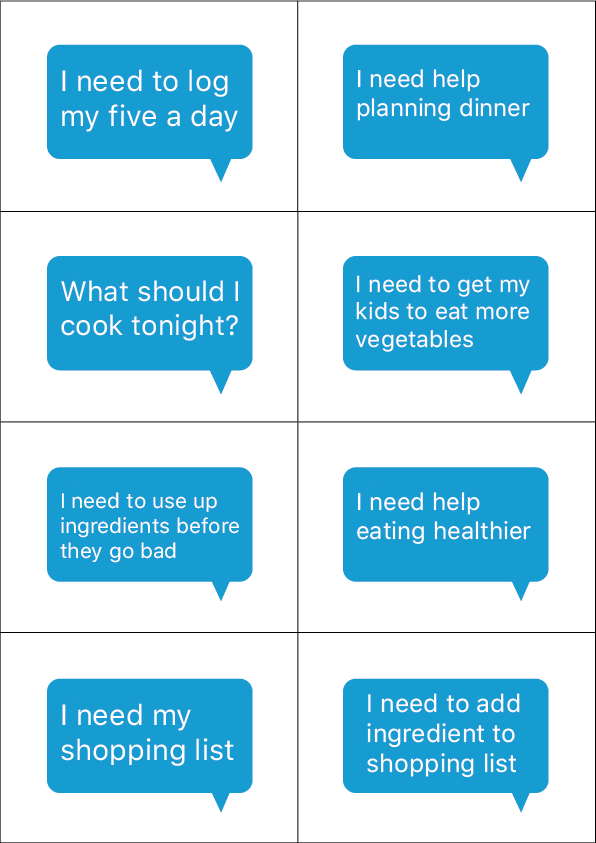
\includegraphics[scale=0.5]{figures/userneeds.png}
            \caption{Figure showing the eight cards with a need to be solved by the chatbot}
            \label{fig:userneed}
        \end{figure}
        
    \begin{figure}[h]
            \centering
            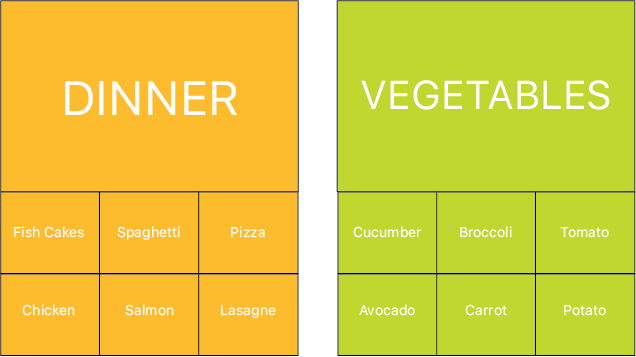
\includegraphics[scale=0.5]{figures/dinnerveg.png}
            \caption{Figure showing the cards for dinners and vegetables}
            \label{fig:dinnerveg}
        \end{figure}
        
     \begin{figure}[h]
            \centering
            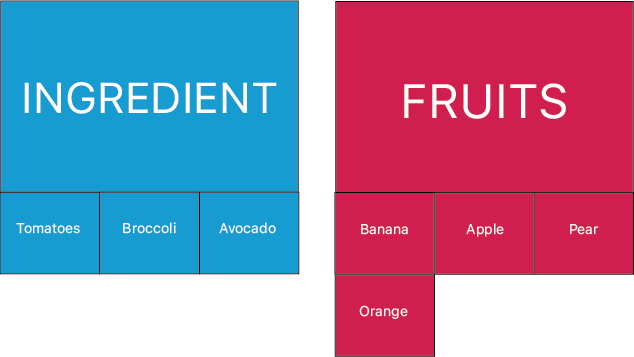
\includegraphics[scale=0.5]{figures/Ingredientfruit.png}
            \caption{Figure showing the cards for ingredients and fruits}
            \label{fig:ingfruit}
        \end{figure}

   The decks were necessary to exclude any interference from the researcher, and also ensured that participants were engaged in conversations flows that the chatbot had been trained to know well. This allowed the researcher to focus on only eight specific conversations to allow participants to interact with the system. The preliminary study conducted as preparation for this master project found that users need a goal with the interaction and expect a chatbot to be able to do something, or perform some kind of service, to perceive the interaction as meaningful. Participants were unable to give a true evaluation of their perception in the preliminary study if they did not "see the point" with the interaction, although the questions were to assess the personality. Therefore, participants will use the chatbot as intended, although the research aim is not to assess how well the chatbot performs its tasks, or whether users find the specific features as more or less valuable to them.
   
   Half of the group will test chatbot A first, while the second half will test chatbot B first. This is to avoid reactivity where users will become familiar with the interface, and therefore feel more at ease when interacting with the second chatbot. After the participants have interacted with each chatbot they will be asked to assess the chatbot personality characteristics to determine whether participants are in agreement regarding the perceived characteristics and personality traits. Then participants will be asked to fill out the AttrakDiff evaluation to assess the perceived hedonic- and pragmatic quality and attractiveness of the chatbot, before repeating the same process with the second chatbot version. This experiment setup will ensure statistic power, as it will allow each participant to be evaluated with themselves.
    

   